In recent years, there has been an enormous development of the field of multi-agent systems. More and more complicated systems have been designed, in order to mimic the motion of animals, which operate in swarms. Some of these animals can be seen in the figures \ref{fig:1.1}, \ref{fig:1.2} and \ref{fig:1.3}. In addition, these structures are complex and difficult to solve, so a different approach was developed in order to analyze them. The concept of the method is to decouple the system into sub systems, who communicate with each other through their links. These connected subsystems have been defined as a distributed system.     

\begin{figure}[H]
    \centering
    \begin{minipage}{.5\textwidth}
        \centering
        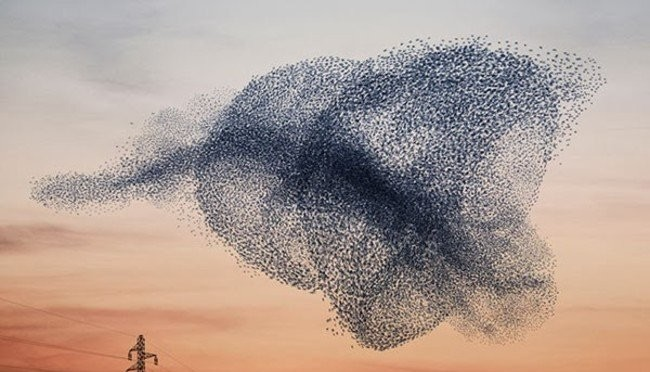
\includegraphics[width=0.8\linewidth]{images/Chapter1/Swarm birds.jpg}
        \caption{A flock of birds.}
        \label{fig:1.1}
    \end{minipage}%
    \begin{minipage}{.5\textwidth}
        \centering
        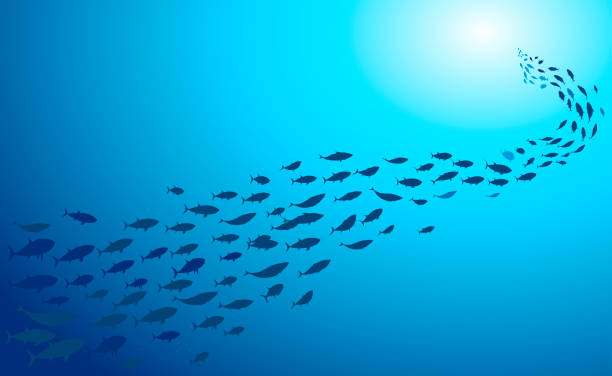
\includegraphics[width=0.8\linewidth]{images/Chapter1/Swarm fish.jpg}
        \caption{A swarm of fish.}
        \label{fig:1.2}
    \end{minipage}
        \begin{minipage}{.5\textwidth}
        \centering
        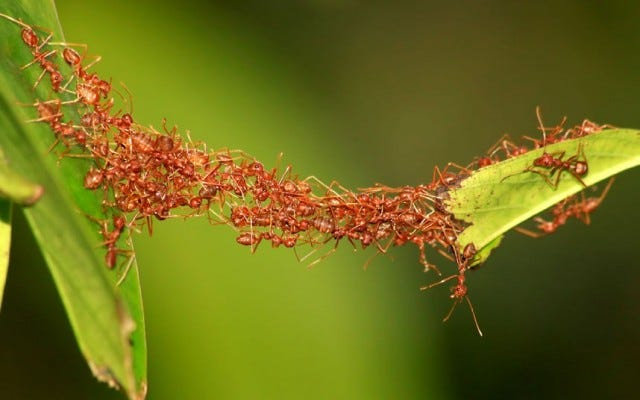
\includegraphics[width=0.8\linewidth]{images/Chapter1/Ant Swarm.jpg}
        \caption{A swarm of ants constructing a bridge.}
        \label{fig:1.3}
    \end{minipage}
\end{figure}

\newpage

A distributed system is a graph based architecture in which the nodes are the agents and the edges are the communication channels. Through the channels, each agent transmits and receives the data distributedly to his neighbor and vice versa. A representation of the architecture can be seen in figure \ref{fig:1.4}. A great application of the multi-agent systems is the consensus problem. According to the problem, the agents converge to a similar desired state, based on constraints of the information exchange between the agents of the network. According to \cite{1239709}, there have been developed a variety of consensus protocols. These protocols were developed in order to mimic the motion and the perception of swarms. So, the agents have a similar behavior to a swarm, thus achieving a desired goal, which was set, as a group.

\begin{figure}[H]
    \centering
    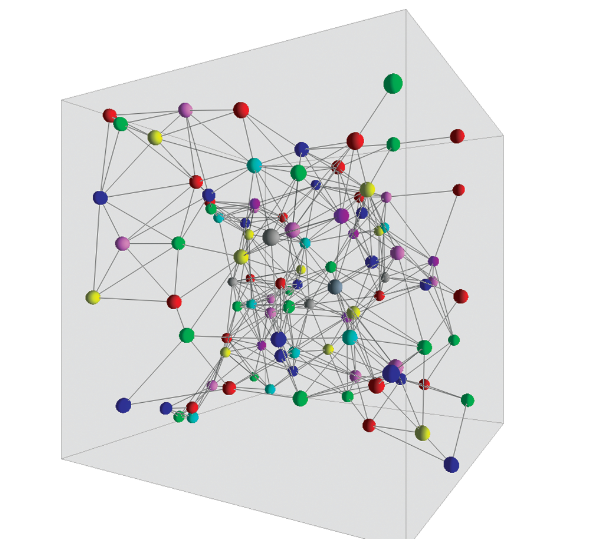
\includegraphics[width=0.3\linewidth]{images/Chapter1/Distributed network.png}
    \caption{Architecture of a distributed network.}
    \label{fig:1.4}
\end{figure}

In order to achieve consensus, the distributed system must receive specified commands. These commands are produced through a distributed control system. Such systems were designed in order to give specific tasks to agents for execution, \cite{DZW2021},\cite{LZHMD2014}. The field of distributed control attracted a significant number of scientists, leading to the development of novel control techniques. In addition, were developed two different approaches to the problem. The first method was centralized control, which is a master-slave approach. A master agent executes the task and exchanges local information with the other agents. The other agents follow the instructions given by the central agent. The second method of control is defined as decentralized or distributed. In this method, every agent acts based on local information which is available. The agents execute the desired tasks while exchanging information with their neighbors. Although, distributed control has a complex form, it is also a more realistic approach for appliance. As a result, physical systems have limitations, such as restricted range in communications, due to finite bandwidth and the number of the agents that exist in the network.

Recently, a number of issues have occurred regarding the distribution of the resources in various fields of applications, such as machine learning and automatic control. The answer to this problem comes from the area of distributed optimization. In particular, the optimal consensus problem is a reliable solution. The optimal consensus problem can be solved with cooperative control techniques and a distributed optimization problem. Therefore, every agent is equipped with a local cost function. Furthermore, agents are assigned to minimize the summation of these cost functions with respect to the constraints of the problem, while exchanging local information in intervals of time, \cite{DZW2021}.

The study of multi-agent systems led to the utilization of distributed optimization and distributed control techniques, in order to design robust methods. These results will not only lead to optimal solutions for current unsolved problems, but also for future ones.


\section{Motivation and Contribution}

The aim of this thesis is to solve the proximal optimal consensus problem, with non-convex constraints, for quadcopters who exchange partial information of their position with their neighbors, which are obtained at sampled periods of time. In addition, the algorithm will lead the agents in the region of the optimal point. In order to achieve this goal, NOn-Convex Gradient PROXimal (NOCGPROX) variables were defined, which are added into the Prox-GPDA algorithm, \cite{pmlr-v70-hong17a}, to prove the proximal optimal consensus. The development of robust distributed control laws that guarantee square integration of NOCGPROX variables is a crucial prerequisite for the convergence of the algorithm. In this manner, will be achieved proximal optimal consensus. Additionally, the quadcopters will be driven to the optimal consensus point. Furthermore, the signals of the closed loop system have to be bounded.

The thesis' contribution can be summarized in the following manner.

    \begin{itemize}
        \item  The NOCGPROX variables have been introduced, which transform the optimal consensus problem into a regulation one. This allows the problem to be solved with distributed control techniques, while achieving proximal optimal consensus, for agents with nonlinear dynamics.
        \item The proposed method for solving the problem depends on sampled filtered output measurements of the agents, thus achieving low frequencies in communication between them. Furthermore, it requires only the knowledge of the Laplacian matrix and the gradient of the local cost functions. In order to have stability in the system, it requires robust distributed control laws which ensures square integration of the variables. This improves the outline of the algorithm in cases in which the optimal solutions are not inside a feasible set.
        \item The design parameters of the algorithm must have large values to ensure sublinear stability of the method. In addition, NOCGPROX variables must tend to zero, to achieve optimal consensus.
    \end{itemize}


\section{Literature Review}

\subsection{Optimal Consensus Problem}
    A lot of scientific studies have been conducted in the years regarding distributed optimization. The foundation of distributed optimization was demonstrated in \cite{1104412}, in which a variety of asynchronous deterministic and stochastic methods have been developed with the use of gradient. From that point on, network systems have been designed and researched, putting into use distributed optimization algorithms for searching the best solution possible, either in discrete or continuous time.

    Regarding the application of distributed optimization in the consensus problem, most researchers have made use of discrete time algorithms in an attempt to reduce computational costs. The concept of the consensus problem has been studied throughout the years, with many scientific papers being published. An interest approach is presented in \cite{9162430}. The consensus between the agents is achieved through an adaptive schema which guarantee boundedness and regulation of the proposed variables with the sampled measurements being delayed. Additionally, in \cite{9785920} and \cite{9477076} is studied the optimal consensus problem. The optimal consensus is being achieved by utilizing a nonlinear PI controller, \cite{PSILLAKIS201911581}, which regulates the proposed variables with few transmissions of output measurements. In \cite{10125000} another solution is proposed, solving a proximal aspect of the optimal consensus problem. The solution is based on EXTRA algorithm for optimization, \cite{ShiEXTRA15}. The proposed variables ensure approximate consensus to a neighborhood of zero. 

\subsection{Convex and Non-Convex Optimization}
    There have been published numerous proposition for optimization algorithms in multi-agent systems. An algorithm whose being studied a lot is Alternating Direction Method of Multipliers (ADMM), \cite{10.1561/2200000016}. In \cite{9146334} has been proposed a different approach to the method. A more relaxed version is being developed which does not require synchronous updates between the agents with the constraints being convex, and achieve linear stability and convergence. On the other hand, in \cite{YANG2022110551} is proposed a proximal form of the algorithm for non-convex and nonsmooth functions. Non-convex problems are often more difficult to solve. On this proposed framework, these distributed optimization problems can be solved, thus achieving convergence.Another proposed methods for ADMM are presented in \cite{8704712} and \cite{wang2018global}. In both of these articles is presented two extension of the ADMM, which solve nonconvex and nonsmooth optimization, achieving global convergence of the state.

    In general, convex distributed optimization problems have been extensively studied and algorithms are currently have been developed, \cite{6358346},\cite{KIA2015254},\cite{10209260},\cite{DAI2020109256},\cite{SEMSARKAZEROONI20082766},\cite{GU20197548},\cite{QIU2016209}, \cite{8812749},\cite{FENG201612},\cite{YANG2018182},\cite{LIN2016120}, \cite{7500070},\cite{8899755},\cite{9316705},\cite{DOMINGUEZGARCIA201533}. While for nonconvex problems, there is a significant lack of solutions. Due to their structure, it is often difficult to find solutions. Fortunately, various methods have been developed in order to solve them. First, a proximate approach based on the primal-dual method is presented in \cite{pmlr-v70-hong17a}. The proposed approach is based on the primal-dual method, where the primal step minimizes a certain approximation of the augmented Lagrangian of the problem, and the dual step performs an approximate dual ascent, \cite{hong2016decomposing}. In addition, this proposed method transforms the nonconvex function into a strongly convex, thus creating a more linearized approach into solving the problem. The primal dual method is also used in \cite{LEI2016110}. Another primal-dual approach has been researched in \cite{7833143}. It is similar to \cite{pmlr-v70-hong17a}, but with different constraints and algorithm analysis. In \cite{7833143} is proposed an Accelerated Distributed Augmented Lagrangian method which has a faster convergent rate than a simple Augmented Lagrangian method. Another approach to solving nonconvex problems was studied by Paolo Di Lorenzo and Gesualdo Scutari in \cite{7398129},\cite{7383778},\cite{7869154}. A new method has been developed, named NEXT, which was the first algorithmic framework for distributed optimization of a sum of nonconvex (possibly and nonsmooth) cost functions. The described method uses a continuous convex approximation technique, which uses dynamic consensus to distribute computation among agents. Each agent first solves a local convex approximation of the non-convex problem (possibly inexactly) and then performs a local averaging operation. In \cite{7807315} was studied a general framework for nonconvex distributed optimization. To achieve convergence, a perturbed method was employed in the analysis, thus achieving optimal consensus among the agents. In \cite{8472181} and \cite{7776843}, two distributed techniques are being presented. In \cite{8472181} uses nonconvex constraints to bound the velocities of the agents with non-uniform position constrains. Based on a switching method is guaranteed boundedness of the state with sampled neighbor information. The same problem is solved in \cite{7776843}, with the only difference being the topology of the graph, which shifts overtime. Another research in nonconvex optimization is presented in \cite{9965620}. The objective is to steer the agents into an optimal point using partial information which is related to input and output. In addition, momentum-based optimal coordinators are design in order to achieve a steady-state. When solving an optimization problem, it is common for the solver to reach a local minimum. This problem is presented in \cite{9246278} with a solution for escaping local optima. The concept is to transform the gradient method into a boosted gradient with nonzero magnitude. Thus, the  optimizer will converge into a global minimum. In \cite{10025380,9462469} is presented a nonconvex framework for solving online the optimization problem using dynamic regrets. In this proposed framework, \cite{FARINA2019243}, is presented an asynchronous distributed approach in which both objective function and constraints are nonconvex. It uses a trigger event on which every node has limited access to the function and the constraints. During that time, the method of multipliers is applied to minimize the Augmented Lagrangian. 

    Most optimization algorithms use gradients to be solved. However, there exists a number of algorithms who are gradient free. These algorithms from their nature are stochastic. An interesting research was conducted by Hajinezhad and Zavlanos in \cite{8619333}, where the distributed nonconvex optimization is being solved without the use of gradient. Their approach is based on a primal dual method, in which every agent has access only to partial information about the global cost function, knowing only the zeroth-order information of their local cost function.

\subsection{Graph Topology Variations}
    While the objective function fulfills a significant role in distributed optimization of the agents, there is another factor that contributes towards the problem. It is also important to consider the topology of the graph. Most of the above mention researches have an undirected topology considering the graph. In \cite{GU20197548}, \cite{DOMINGUEZGARCIA201533}, \cite{9112274}, \cite{6894574}, \cite{9992866} and \cite{YOO2018421} the topology of the graph is directed. The main categorization of the topology lies into static and dynamic graphs. The static graphs have one topology that does not change in time. While dynamic topology (or switching topology) changes in time. Therefore, the matrices and vectors of the problem are time variant. In fact, it's clear from \cite{8340193} that different ways of solving the optimization problem exist, regarding the topology. Throughout the graph is observed the communication tradeoff of the agents. Thus, network topology fulfills a crucial role in the analysis. 

    Although fixed topologies have been extensively studied throughout the years, research has been conducted on switching topologies as well. A thoroughly established illustration of the usage of both fixed and switching topology is studied in \cite{8723151}. A class of distributed nonlinear controllers have been designed in order to achieve consensus for high-order agents in both topologies. In \cite{8445642} a similar approach is presented, but with unknown high frequency gain signs. The method which was proposed assures consensus between the agents with non-identical unknown control directions under the switching graph. A more probabilistic approach is presented in \cite{5404835}. While exchanging packages, the agents change their topology randomly when a packet is lost. As a result, the agents are modelled as a system with a stochastic switching undirected topology, which in conjunction with the proposed algorithm is robust to ensure consensus. Oftentimes, consensus protocols tend to be executed asynchronous between the agents. Such cases are presented in \cite{9244621} and \cite{4631522}. In the first one, a switched observer was designed which estimates the state information of the leader, which is based on a general switching topology rule of the spanning tree of the graph. While feedback distributed control laws ensure consensus in all modes of the graph. The later one, ensures consensus between the agents, while the topology switches during time-delays. In \cite{9736623} is presented a novel approach regarding the losses which occurs during the switching of the topology. This simple approach is base on a high-order filter to generate differentiable control variables using neighbor position information  and discontinuous topology information. Another research paper is presented in \cite{6839031}, which ensures robust consensus tracking control, considering the fact that the topology changes in time with disturbances in the communications. Lastly, in \cite{8100757} is presented an adaptive mechanism which ensures cooperation between the agents under switched topologies. In this paper are presented two distributed event-trigger control schemes, in which the agents track reference inputs asymptotically and reject disturbances. 

\section{Thesis Structure}

This diploma thesis consists of six chapters in total. The first chapter contains the introduction for this thesis and the motivation behind it. In addition, the chapter also contains the review of the literature. The chapter also contains the thesis structure and bibliography.

The second chapter discusses the fundamental mathematical concepts and axioms utilized for proving and designing both the algorithm and the robust distributed control laws.

In the third chapter, the NOCGPROX variables are introduced in order to solve the proximal output consensus. Additionally, it contains a mathematical proof analysis of the algorithm with its lemmas and theorem, which prove proximal consensus.

In the fourth chapter, the nonlinear dynamics of the agents are transformed to incorporate the NOCGPROX variables into the dynamics. The robust distributed control laws are introduced which ensure the square integration of the variables with sliding surface feedback linearization method to ensure that the variables tends to zero and be square integrable.

The fifth chapter is consisted of the simulation of the algorithm and control laws for the agents. In the simulation, there are applied different scenarios in order to achieve optimal consensus of the agents.

The sixth and final chapter contains the concluding remarks of this thesis and purpose, while future research is discussed for improvements of this work.